\documentclass[11pt]{article}
\usepackage[margin=1in]{geometry}
\usepackage{graphicx}
\usepackage{booktabs}
\usepackage{amsmath}
\usepackage{amssymb}
\usepackage{xcolor}
\usepackage[colorlinks=true,linkcolor=blue,citecolor=blue,urlcolor=blue]{hyperref}
\usepackage{caption}
\captionsetup{font=small}

\title{\textbf{Efficient Thinking: Tradeoffs in Game-Playing AI}\\[4pt]
\large Parameters vs.\ Search vs.\ Self-Learning --- a Three-Stage Chess Study\\ of Where Strength Comes From}
\author{Louay Alsakka\\ \small\texttt{louayalsakka@gmail.com}\\
\small Code, trained model, and figures: \url{https://github.com/LouayAlsakka/efficient-thinking}}
\date{July 2026}

\begin{document}
\maketitle

\begin{abstract}
We study how playing strength in chess arises from three separable sources---\textbf{network
capacity, search, and self-learning}---using a deliberately tiny model on modest hardware. A
\textbf{3.45\,M-parameter (14\,MB) convolutional network} plays at $\sim$2150 Elo as a single-pass
policy; adding \textbf{Monte-Carlo Tree Search (MCTS)} lifts the \emph{same weights} to
$\sim$2800-class strength with \textbf{zero extra parameters}---strength bought with compute, not
parameters. We make three further contributions. (1) A direct \textbf{MCTS-vs-fixed-depth}
comparison: adaptive MCTS both beats alpha--beta at equal compute and keeps scaling, while
fixed-depth search plateaus. (2) A \textbf{search-efficiency} result: an all-MCTS wide$\rightarrow$narrow
\emph{cascade} that funnels the simulation budget through progressively narrower, deeper stages
matches flat-MCTS strength while running up to $\sim$4.8$\times$ faster per move. (3) A
\textbf{teacher-free self-learning} study (self-play, a self-referential ladder, evolution, and
committees) with one robust positive and sober negatives: model \emph{agreement} predicts
correctness (a confidence signal needing no oracle), but none of these methods---including
outcome-based evolution---crosses the self-play plateau, and plurality voting does not reliably
de-bias. Since the same network reaches higher under supervised labels, the wall is the quality of
\emph{self-generated} signal, not capacity. Throughout, the unifying finding is that \textbf{the
learned evaluator is the bottleneck}: search and self-play \emph{redistribute} the network's
knowledge; they do not manufacture it.
\end{abstract}

\noindent\textbf{Note on numbers.} Absolute Elo is measured against a Stockfish ladder and carries
systematic uncertainty ($\pm$100) near the top rung; the \emph{relative} results (MCTS-vs-fixed, the
cascade curve, the Stage-3 negatives) are the robust claims, and ``$\sim$2800'' is an efficiency
indicator, not an engine-matching claim.

\section{Introduction}
Modern game AI conflates three separable questions: (1)~\emph{open loop}---how strong is a single
forward pass (pure ``intuition'')? (2)~\emph{closed loop}---how much does search (lookahead on a
learned value function) add? (3)~\emph{self-learning}---can the system improve itself with no
external teacher? We treat these as three stages of increasing autonomy and measure each
independently. The framing is control-theoretic~\cite{bertsekas2022lessons}: the open-loop policy is
a feedforward controller, closed-loop search is model-predictive control (receding-horizon planning
with a learned terminal cost), and self-play is iterative/adaptive learning control. Chess is only a
testbed; the goal is a generic recipe for sequential decision-making.

\paragraph{Contributions.}
\begin{itemize}\itemsep2pt
\item A parameter-efficiency result: $\sim$2800 Elo from 3.45\,M parameters via search, at constant memory.
\item A direct \textbf{MCTS-vs-fixed-depth} result: adaptive search beats and out-scales fixed depth.
\item A \textbf{search-efficiency} result: a wide$\rightarrow$narrow MCTS cascade matches flat MCTS at up to $\sim$4.8$\times$ less compute per move.
\item An \textbf{architecture-beats-scale} finding (convolution $\gg$ MLP at equal data).
\item A reproducible \textbf{negative result} on small-scale self-learning: self-play, a self-referential ladder, evolution, and plurality-voting committees all fail to cross the plateau, with a methodological warning that noisy fitness manufactures phantom gains.
\end{itemize}

\section{Problem Setup and Methods}
\paragraph{Representation.} Position$\rightarrow$move as a 4096-way ($64\times64$ from--to)
classification; promotions default to queen. The board is always presented from the mover's
perspective (mirror $+$ color-swap for Black), so one network serves both players. Encoding:
64 squares $\times$ 12 piece planes $+$ 5 meta bits $=$ 773 floats; for convolution this reshapes to
$8\times8\times12$ piece planes $+$ 5 meta planes ($=17$ input channels).

\paragraph{Labels and objective.} Supervised data is the public Lichess cloud-eval database
($\sim$394\,M positions), each with Stockfish multi-PV win-probabilities. The \emph{hard} objective
is cross-entropy to the single best move; the \emph{soft} objective is cross-entropy to an
advantage-weighted distribution over legal moves ($\mathrm{softmax}(v_i/\tau)$), which is not
bounded by copying one move and generalizes better.

\paragraph{Evaluation.} Elo via a Stockfish ladder (random baseline, then Stockfish at set
\texttt{UCI\_Elo} rungs), fit by maximum likelihood against the known rung ratings. If the player
beats the top rung the estimate compresses, so we raised the ladder as the player improved
($1700\rightarrow2100\rightarrow2700\rightarrow3000$); relative gains on the \emph{same} ladder are
the robust results. Where two methods are compared they are always run on the same ladder, seeds,
and openings.

\paragraph{Hardware.} Two Apple-Silicon Mac Studios (M3 Ultra, 256\,GB each), MLX
framework~\cite{mlx2023}, 40\,Gbps bridge.

\section{Stage 1 --- Open Loop (single-pass policy)}
\paragraph{Topology sweep.} At fixed data (18\,M positions) we swept eight architectures
(Table~\ref{tab:topo}). Only two shapes are competitive---constant-width and convolution---and every
taper, factoring, or exotic bottleneck loses badly, because a taper destroys positional information
before the head can use it while convolution reuses local tactical patterns across the board via
weight sharing. A 3.45\,M-parameter conv matched a 14.4\,M-parameter MLP using $22\times$ less data:
architecture, not parameter count, sets the strength.

\begin{table}[t]\centering\small
\begin{tabular}{lrrl}
\toprule
Topology & Params & Elo & Note \\
\midrule
\textbf{conv (64$\times$10 / 96$\times$8)} & 2.8--3.4\,M & \textbf{1476} & best \& most efficient \\
constant-width MLP (1024$\times$6) & 10.2\,M & 1108--1233 & best plain MLP \\
dual-path (wide+deep, gated) & 2.8\,M & 1082 & ties MLP at 3.5$\times$ fewer params \\
factored head (from/to) & 6.2\,M & 782 & $-450$ \\
funnel (1024$\rightarrow$64) & 1.8\,M & 582 & narrowing hurts \\
pyramid (64$\rightarrow$1024) & 5.0\,M & 431 & bad \\
bottleneck (512$\rightarrow$8) & 0.5\,M & 340 & broken \\
\bottomrule
\end{tabular}
\caption{Topology sweep. Convolution wins overall; tapers and bottlenecks collapse.}
\label{tab:topo}
\end{table}

\paragraph{Scaling and ceiling.} Width shows sharply diminishing returns (W1024$\rightarrow$1449;
W2048$\rightarrow$1501: $+52$ Elo for $3.3\times$ params). Data scaling saturates near the
database's 394\,M limit (Figure~\ref{fig:datascaling}). The soft objective beats hard by
$+94$--$113$ Elo. The best open-loop recipe (conv $+$ soft $+$ full data) has a ceiling
$\approx2150$ Elo at 3.45\,M params, 14\,MB, $\sim$176\,MFLOP / $\sim$1.5\,ms per move---cheap, but
capped.

\begin{figure}[t]\centering
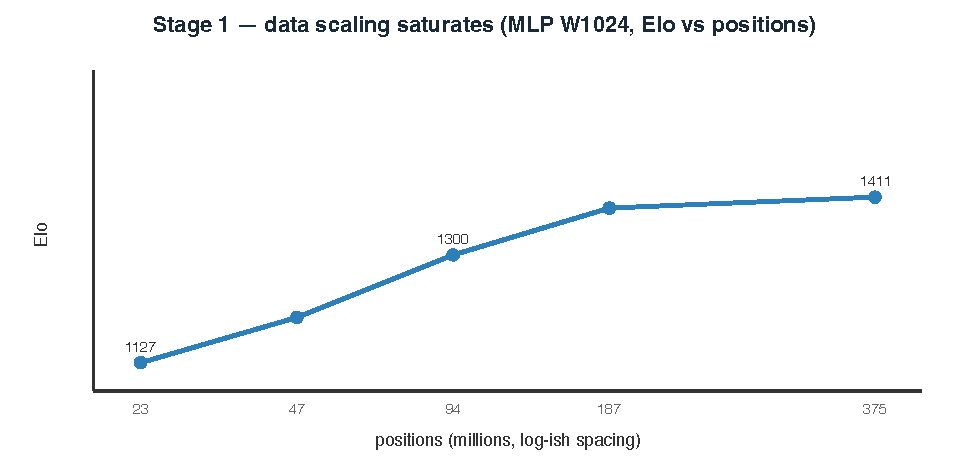
\includegraphics[width=0.72\linewidth]{figs/fig_datascaling.pdf}
\caption{Stage 1: single-pass strength saturates with data (MLP W1024).}
\label{fig:datascaling}
\end{figure}

\section{Stage 2 --- Closed Loop (search on a value function)}
We add a scalar head $\mathrm{Eval}(N)\in[0,1]$ $=$ expected score for the side to move, trained on
the eval-DB win-probabilities (held-out MAE 0.088, correlation 0.877). Search uses the zero-sum
complement identity: our value after a move is $1-\mathrm{Eval}(\text{child})$, so one network plays
both sides; terminal nodes return exact $0/0.5/1$.

\paragraph{MCTS vs.\ fixed depth.} Fixed-depth alpha--beta (with policy move-ordering and
quiescence) rises then plateaus $\sim$2550; 1-ply search actually \emph{hurts} a strong policy
($-34$ Elo, it commits to a capture without seeing the recapture). Adaptive MCTS/PUCT both beats
alpha--beta at equal compute and keeps scaling to $\sim$2800 (Table~\ref{tab:search},
Figure~\ref{fig:mcts}). Fixed uniform depth spends the same effort on every branch and amplifies the
value net's noise at the leaves; MCTS allocates search adaptively to sharp lines and averages over
that noise.

\begin{table}[t]\centering\small
\begin{minipage}{0.48\linewidth}\centering
\begin{tabular}{crr}
\toprule
depth & raw & search \\ \midrule
1 & 1661 & 1627 \\
2 & 1685 & 1788 \\
3 & 1895 & 2005 \\
4 & 1914 & 2152 \\
6 & 2128 & \textbf{2575} \\
7 & 2187 & 2513 \\
\bottomrule
\end{tabular}
\\[2pt]\footnotesize alpha--beta (plateau $\sim$2550)
\end{minipage}\hfill
\begin{minipage}{0.48\linewidth}\centering
\begin{tabular}{cr}
\toprule
sims & search Elo \\ \midrule
100 & 2411 \\
200 & 2530 \\
400 & 2610 \\
\textbf{800} & \textbf{2749 ($\sim$2800)} \\
\bottomrule
\end{tabular}
\\[2pt]\footnotesize MCTS (keeps rising)
\end{minipage}
\caption{Fixed-depth search plateaus; MCTS out-scales it on the same value net and ladder.}
\label{tab:search}
\end{table}

\begin{figure}[t]\centering
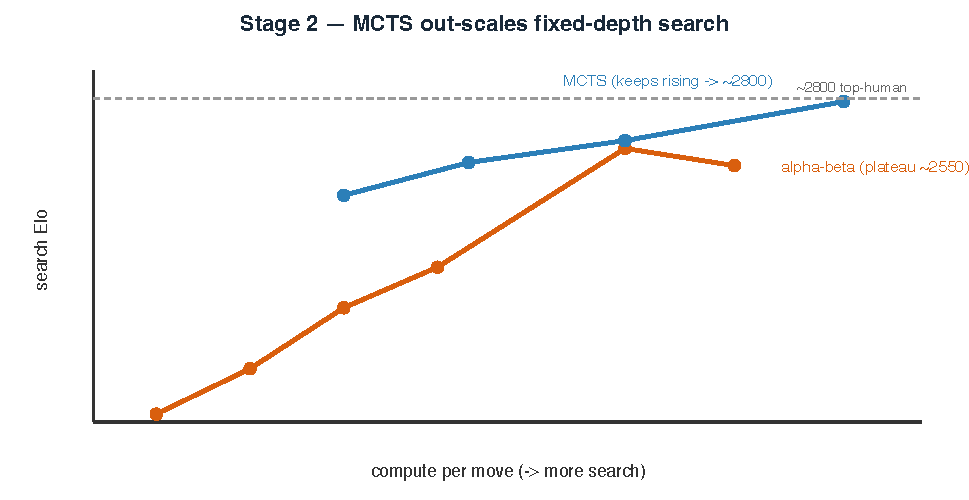
\includegraphics[width=0.72\linewidth]{figs/fig_mcts_vs_fixed.pdf}
\caption{Stage 2: MCTS beats and out-scales fixed-depth search.}
\label{fig:mcts}
\end{figure}

\paragraph{Search efficiency --- the cascade.} Given that MCTS wins, we ask whether the
\emph{allocation} of a fixed simulation budget matters. The cascade runs MCTS in stages with
different knobs: a wide stage (all moves, high $c_{\text{puct}}$, few sims) ranks broadly and passes
its top-$k$ by visit count to a narrower, deeper stage, funnelling the budget onto the survivors
(shared evaluation cache across stages). A controlled $N=1\!\rightarrow\!10$ sweep (all 800 total
sims; same ladder) shows the Elo stays inside a single $\pm$89 noise band (range 2506--2683, mean
$\sim$2580)---statistically flat---while speed improves monotonically to $4.8\times$ at $N=10$
(Figure~\ref{fig:cascade}). Funnelling the budget wide$\rightarrow$narrow is therefore a near-pure
efficiency win: the survivors that reach the deep stages are the same moves flat MCTS would have
spent its budget on anyway. (A fixed-depth \emph{beam} cascade, by contrast, is a genuinely weaker
primitive at 2487---adaptive MCTS stages matter.)

\begin{figure}[t]\centering
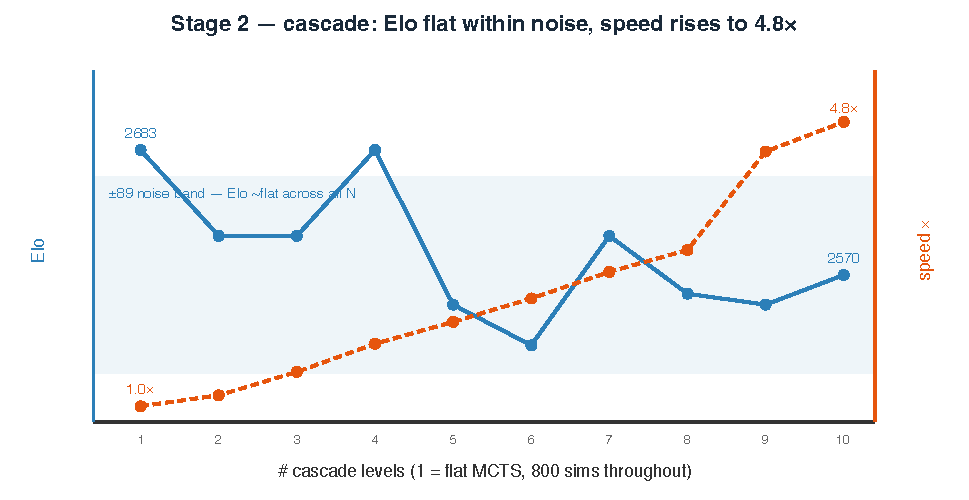
\includegraphics[width=0.72\linewidth]{figs/fig_cascade.pdf}
\caption{Stage 2: the wide$\rightarrow$narrow cascade holds Elo (within noise) while cutting per-move compute up to $4.8\times$.}
\label{fig:cascade}
\end{figure}

\paragraph{Two-dimensional cost.} Stage 1 buys Elo with \emph{memory} and saturates ($\sim$2150,
14\,MB, one pass); Stage 2 buys Elo with \emph{GPU cycles} and keeps climbing ($\sim$2800, 14\,MB,
$\sim$800 passes $\approx$1\,s---or $\sim$0.6\,s cascaded). Strength is compute, not parameters.

\section{Stage 3 --- Self-Learning (no external engine, no labels)}
Stages 1--2 leaned on Stockfish labels, which only exist because chess already has a superhuman
evaluator and a labeled database. The generic goal is the opposite: a new field where \emph{no
training data and no evaluator exist}---a novel game, an unsolved control problem, a design task. There
you cannot imitate a teacher and cannot score positions with an off-the-shelf engine; the only input
is the environment's rules. Stage 3 discards every external crutch to test whether strength can be
bootstrapped from self-play and outcomes alone---the transferable question, since Stages 1--2 are
simply unavailable for a genuinely new problem.

\paragraph{Self-play.} AlphaZero-style expert iteration~\cite{silver2018alphazero}
(MCTS self-play $\rightarrow$ train toward visit-distribution policy $+$ game-outcome value
$\rightarrow$ repeat). Two failure modes appeared and were fixed (cold-start draw-collapse; warm-start
catastrophic forgetting), but the raw policy plateaus $\sim$1950--2030---below the $\sim$2150
supervised baseline (Figure~\ref{fig:selfplay}). Self-play strength does rise with game volume, but
the achievable volume here plateaus under a 394\,M-supervised net; scale is the binding constraint.

\begin{figure}[t]\centering
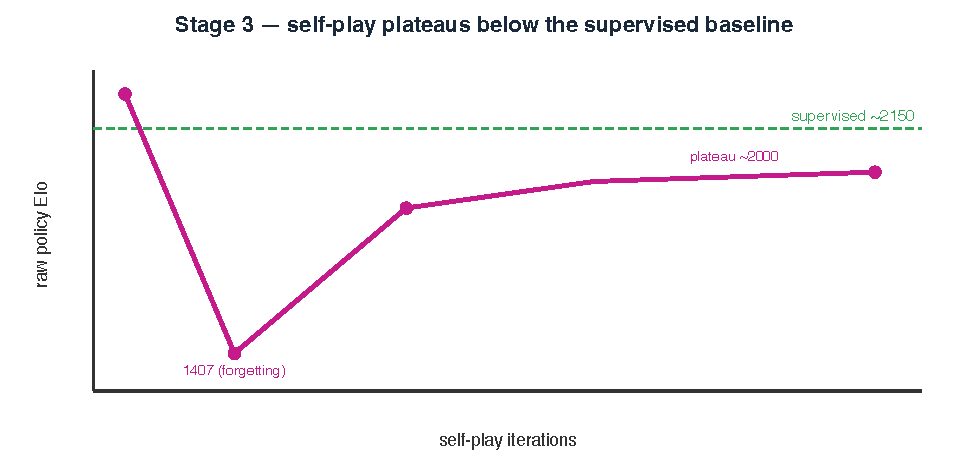
\includegraphics[width=0.68\linewidth]{figs/fig_selfplay.pdf}
\caption{Stage 3: self-play plateaus below the supervised baseline.}
\label{fig:selfplay}
\end{figure}

\paragraph{Committee / diversity.} If the bottleneck is the evaluator, a cheap way to improve one
without a bigger net is to ensemble diverse nets. We tested whether multiple independently-trained
models diverge (disagree $\Rightarrow$ uncertain) or converge (agree $\Rightarrow$ likely correct).
\emph{Agreement strongly predicts correctness} (Figure~\ref{fig:agreement}): over 400 positions
scored against Stockfish depth-12, unanimity reaches 65--94\% top-move accuracy vs.\ 17--37\% when
members disagree---a validated, self-contained confidence meter. However, plurality \emph{voting}
does not reliably de-bias: across a committee-size sweep (Table~\ref{tab:csize},
Figure~\ref{fig:csize}) the consensus is slightly \emph{worse} than the best single member at every
size (gaps within the $\sim\pm$3\,CPL measurement noise), \emph{balance beats count} (adding
correlated same-family members lets that bloc dominate the vote and reverts the gain), and the
per-position oracle is $2$--$3\times$ better than the vote---the diversity contains the information,
but plurality cannot extract it.

\begin{table}[t]\centering\small
\begin{tabular}{lrrr}
\toprule
agents & consensus CPL & best member & oracle \\ \midrule
3 (conv-soft $\times$3) & 54.7 & 49.8 & 29.6 \\
5 (+MLP +hard) & \textbf{48.0} & 46.8 & 22.2 \\
7 (+2 data-slice conv) & 54.8 & 52.2 & 20.8 \\
9 (+MLP +hard) & 56.0 & 53.1 & 19.9 \\
\bottomrule
\end{tabular}
\caption{Committee-size sweep (centipawn loss, lower better). Plurality never clearly beats the best member; balance ($N{=}5$) beats count; the oracle headroom is unrealized.}
\label{tab:csize}
\end{table}

\begin{figure}[t]\centering
\begin{minipage}{0.49\linewidth}\centering
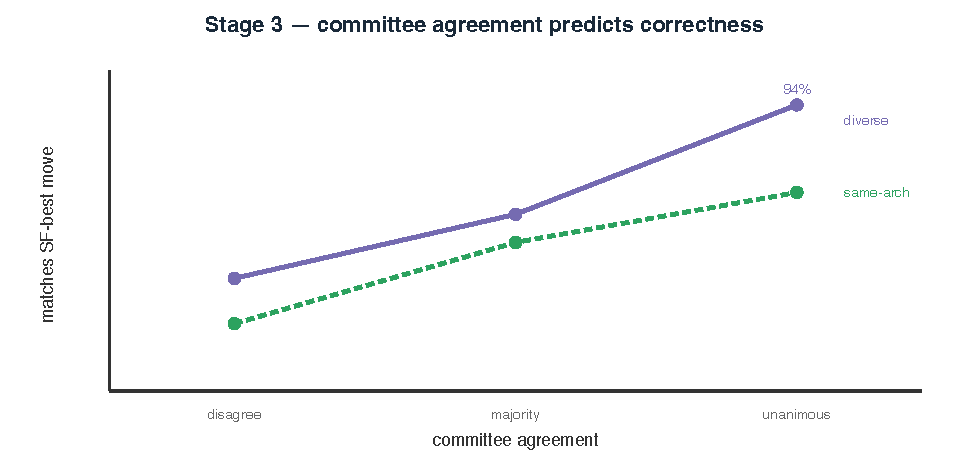
\includegraphics[width=\linewidth]{figs/fig_agreement.pdf}\end{minipage}\hfill
\begin{minipage}{0.49\linewidth}\centering
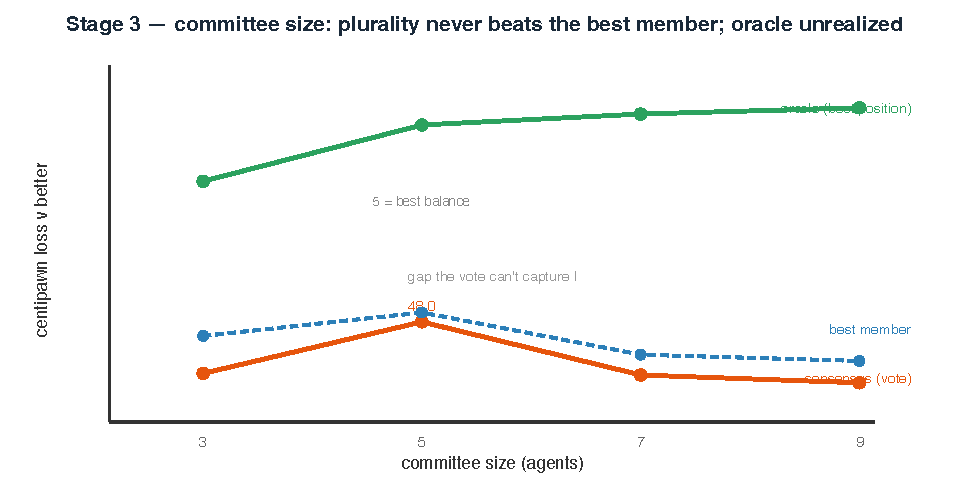
\includegraphics[width=\linewidth]{figs/fig_committee_size.pdf}\end{minipage}
\caption{Left: committee agreement predicts correctness (robust). Right: plurality voting never beats the best member, and adding correlated members reverts the gain.}
\label{fig:agreement}\label{fig:csize}
\end{figure}

\paragraph{Evolution (mutate / play / score).} Gradient self-play optimizes a proxy (the net's own
biased value targets); we tested whether derivative-free evolution, optimizing the true
objective---did this mutant win games---could escape the plateau. From the plateaued net, each
generation mutates it into 16 offspring (Gaussian weight noise), plays each against a \emph{frozen
copy of the plateaued net} (a fixed anchor, so ``fitness'' is ``how well do you beat the plateau''),
and crowns the best only if it survives a larger confirmation match. A naive version selecting
against the \emph{moving} champion drifted downward---beating your immediate parent is
non-transitive in chess. \textbf{The result is a null result and a methodological warning}
(Figure~\ref{fig:evolution}): the run \emph{appeared} to escape ($+47$ Elo, passing a 120-game
confirmation), but a clean 400-game low-temperature re-match found the ``evolved'' champion is
actually $-24$ to $-41$ Elo \emph{worse}---a phantom improvement from noisy, high-temperature fitness
with best-of-16 selection bias. Annealing the mutation scale up ($\sigma\!:\!0.03\!\rightarrow\!0.12$)
found nothing better. So evolution did not escape either, and neither gradient self-play, a
self-referential ladder, nor evolution crosses the $\sim$2000 wall.

\begin{figure}[t]\centering
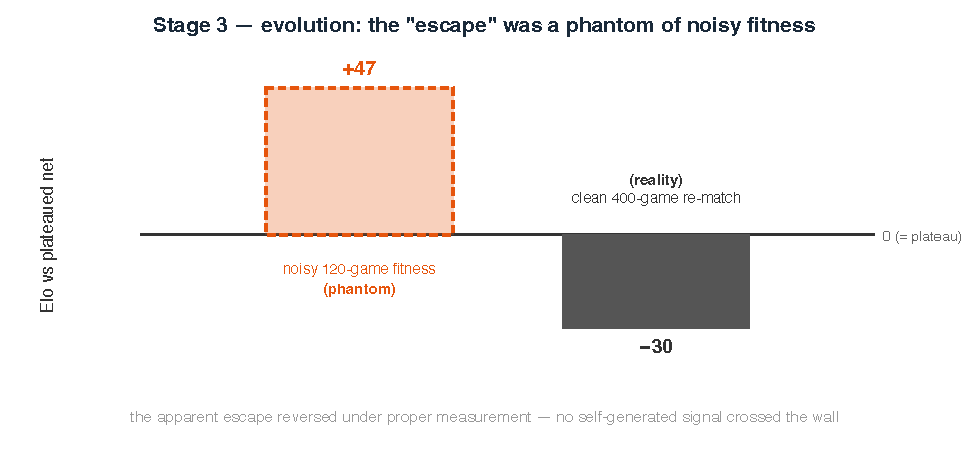
\includegraphics[width=0.62\linewidth]{figs/fig_evolution.pdf}
\caption{Stage 3: the evolution ``escape'' was a phantom---noisy fitness said $+47$ Elo, a clean re-match said $-30$.}
\label{fig:evolution}
\end{figure}

\section{Comparison to Existing Systems}
Our net is $\sim$10--25$\times$ smaller than AlphaZero and 30--100$\times$ smaller than large Leela
transformers~\cite{lc0,silver2018alphazero,mcilroy2020maia,stockfishnnue}, yet reaches $\sim$2800
with search---the extreme point on Elo-per-parameter (Figure~\ref{fig:paramefficiency}). The two
paradigms differ in speed: AlphaZero/Leela use a similar sim count but each sim is a big-net pass,
so their per-move cost is dominated by a $10$--$100\times$ larger network; Stockfish is the opposite
regime---a small quantized net at millions of alpha--beta nodes/second. The common structure:
strength $=$ evaluator $\times$ search; every strong engine is search-heavy, and parameter count is
not what separates them. (Honest gap: top engines are $\sim$600--800 Elo above $\sim$2800, from far
more search \emph{and} a much better value net.)

\begin{figure}[t]\centering
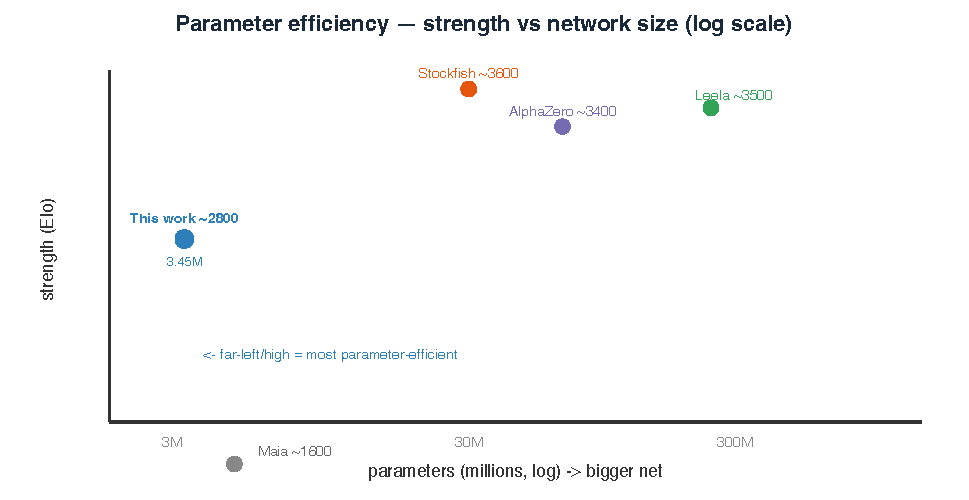
\includegraphics[width=0.68\linewidth]{figs/fig_paramefficiency.pdf}
\caption{Parameter efficiency: strength vs.\ network size (log scale). This work is the far-left/high (most efficient) point.}
\label{fig:paramefficiency}
\end{figure}

\section{Discussion}
Across all three stages one result recurs: \textbf{the ceiling is the evaluator, not the loop around
it.} (i)~\emph{Architecture $>$ parameters}: the right prior beats raw width. (ii)~\emph{Search $>$
scale, at constant memory---but search cannot exceed the net}: flat MCTS and the cascade hit the same
$\sim$2691 wall on the same ladder because they query the same value net; search reduces the net's
\emph{variance} (via averaging) but not its \emph{bias}, and deep uniform search even amplifies bias.
(iii)~\emph{No self-generated signal crosses the wall---we tried three}: gradient self-play, a
self-referential ladder, and evolution all fail, and since the same net reaches $\sim$2150 under
supervised labels the wall is not capacity but the ceiling of any signal a system generates about
\emph{itself}. (iv)~\emph{A better evaluator is the only lever---but it is harder than it looks}: the
committee gives a robust confidence signal, yet plurality voting does not reliably de-bias; capturing
the oracle headroom needs a better aggregator (soft-averaging / confidence routing) and balanced,
not merely numerous, diversity.

\section{Limitations and Future Work}
Absolute Elo carries systematic uncertainty near the ladder top; relative same-ladder gains are the
robust claims. Stage 3 is compute-limited (two machines) and characterizes the small-scale regime;
relative-fitness selection with small stochastic samples produced a phantom evolution ``escape'' that
reversed under a 400-game re-match, and plurality de-biasing gaps sit inside the measurement noise.
Priorities: (1)~a better value function---the true ceiling---via more/better search-labeled data or
large-scale self-play; (2)~a better ensemble \emph{aggregator} (soft-averaging, confidence routing)
with balanced cross-family diversity; (3)~batched/parallel MCTS and transposition tables; (4)~endgame
tablebases and tuned $c_{\text{puct}}$.

\section{Conclusion}
A 14\,MB, 3.45\,M-parameter network reaches $\sim$2800-class chess strength by \emph{thinking} (MCTS
search), not by \emph{growing} (parameters); adaptive MCTS beats and out-scales fixed-depth search;
and a wide$\rightarrow$narrow cascade matches it at up to $4.8\times$ less compute. On the
self-learning side the results are honestly negative: self-play, a self-referential ladder, and
evolution all fail to cross the $\sim$2000 plateau (evolution's apparent escape was a noise
artifact), and plurality-voting committees do not reliably de-bias---though model agreement is a
robust teacher-free confidence signal. The transferable result, proven from every direction we
pushed, is that the learned evaluator is the bottleneck: search redistributes its knowledge and
self-generated signal cannot exceed its own quality; only a better evaluator raises the ceiling.

\bibliographystyle{plain}
\bibliography{refs}
\end{document}
